%\documentclass[a4paper,doc]{apa6}
\documentclass[a4paper]{article}
% \graphicspath{{/figures/}{./../figures/}}

\usepackage[english]{babel}
\usepackage[utf8x]{inputenc}
\usepackage[colorlinks=true, urlcolor=blue, citecolor=blue, linkcolor=blue]{hyperref}

\usepackage{apacite}
\usepackage{authblk}  % for authors
\usepackage{xcolor}
\definecolor{mypink}{RGB}{255, 230, 255}

\usepackage{nicefrac}
\usepackage{amsmath}
\usepackage{graphicx}
\usepackage{chngcntr} % appendix references
\usepackage[colorinlistoftodos,prependcaption]{todonotes}
\usepackage{pgfplotstable}
\pgfplotstableset{
	fixed zerofill,
	precision=3,
	col sep = comma,
	search path={../tables/}
}
\pgfkeys{/pgf/number format/precision=2, /pgf/number format/fixed}%

\newcommand{\getValue}[3]{%
	\pgfplotstablegetelem{#1}{#2}\of{#3}%
	\pgfmathprintnumber{\pgfplotsretval}%
}
\newcommand{\setValue}[4]{%
	\pgfplotstablegetelem{#1}{#2}\of{#3}%
	\pgfmathprintnumberto{\pgfplotsretval}{#4}%
}


\newcommand{\getCI}[2]{[\getValue{#1}{Lower}{#2}, \getValue{#1}{Upper}{#2}]}

\usepackage{titlesec}

\titlespacing\section{0pt}{8pt plus 4pt minus 2pt}{4pt plus 2pt minus 2pt}
\titlespacing\subsection{0pt}{8pt plus 4pt minus 2pt}{0pt plus 2pt minus 2pt}
\titlespacing\subsubsection{0pt}{8pt plus 4pt minus 2pt}{0pt plus 2pt minus 2pt}

\usepackage{tikz}
\usepackage{tikzscale} % check if used!

\usepackage[most]{tcolorbox}

\newtcolorbox[auto counter]{NewBox2}[2][]{
	colframe=black,colback=white,
	enhanced,
%	breakable,
	title={Box \thetcbcounter: #2},
	colbacktitle=white,
	coltitle = black,
	detach title,
	before upper={\tcbtitle\quad},
	#1
}
%\getValue{0}{ph0}{\reanalysis}

\newcommand{\EJ}[1]{\todo[inline, color=green]{  #1 }}
\newcommand{\Q}[1]{\todo[inline, color=yellow]{  #1 }}
\newcommand{\jv}[2]{{\color{red}\st{#1}}{\color{blue}\bf{#2}}}
\newcommand{\DON}[1]{\todo[inline, color=white]{Don: #1}}
\newcommand{\DONside}[1]{\todo[color=white]{#1}}
%\newcommand{\DONTODO}[1]{{\color{red}{#1}} \addcontentsline{tdo}{todo}{#1}}
\newcommand{\J}[1]{\todo[inline, color=mypink]{#1}}

\graphicspath{{../figures/}}
\newcommand{\hypo}[1]{\ensuremath{\mathcal{H}_{#1}}}
\newcommand{\model}{\mathcal{M}}
\newcommand{\data}{\mathrm{data}}%\mathcal{D}}
\newcommand{\midd}{\ensuremath{\,|\,}}
\newcommand{\cohend}{\ensuremath{d}}
\newcommand{\prob}{\mathrm{Pr}}

\newcommand{\osflink}{\url{https://osf.io/uq8st/}}

\newcommand{\CamererReplication}{\url{https://mfr.osf.io/render?url=https://osf.io/fg4d3/?action=download\%26mode=render}}
\newcommand{\manyLabsLink}{\url{https://mfr.osf.io/render?url=https://osf.io/xufw4/?action=download\%26mode=render}}


\title{A Cautionary Note on Estimating Effect Size}
%\shorttitle{Estimating Effect Size} 
\renewcommand{\thefootnote}{\fnsymbol{footnote}}
\author[1]{Don van den Bergh%
	\thanks{Correspondence concerning this article should be addressed to: Don van den Bergh, University of Amsterdam, Department of Psychological Methods, Nieuwe Achtergracht 129B, 1018VZ Amsterdam, The Netherlands. E-Mail should be sent to: donvdbergh@hotmail.com.
}}
\author[1]{Julia M. Haaf}
\author[1,2]{Alexander Ly}
\author[3]{\authorcr Jeffrey N. Rouder} % putt Jeff on a newline to avoid a newline after his first name
\author[1]{Eric-Jan Wagenmakers}
\affil[1]{University of Amsterdam}
\affil[2]{Centrum Wiskunde \& Informatica}
\affil[3]{University of California Irvine}
\date{}
%\affiliation{~}
\renewcommand*{\thefootnote}{\arabic{footnote}}
%
%\threeauthors{Don van den Bergh and Julia M. Haaf and Alexander Ly and Eric-Jan Wagenmakers}{Alexander Ly}{Jeffrey N. Rouder}
%\threeaffiliations{University of Amsterdam}{Centrum Wiskunde \& Informatica}{University of California Irvine}
%\authornote{Correspondence concerning this article should be addressed to: Don van den Bergh, University of Amsterdam, Department of Psychological Methods, Nieuwe Achtergracht 129B, 1018VZ Amsterdam, The Netherlands. E-Mail should be sent to: donvdbergh@hotmail.com.}

\pgfplotstableread{effectSizeExample.csv}\tbEffectSizeExample
\pgfplotstableread{posteriorProbH0.csv}\reanalysis

\begin{document}

%\listoftodos
%\newpage

\maketitle

\begin{abstract}
	An increasingly popular approach to statistical inference is to focus on the estimation of effect size while ignoring the null hypothesis that the effect is absent. We demonstrate how this common ``null hypothesis neglect'' may result in effect size estimates that are overly optimistic. The overestimation can be avoided by incorporating the plausibility of the null hypothesis into the estimation process through a ``spike-and-slab'' model.
\end{abstract}

Consider the following hypothetical scenario: a colleague from the biology department has just conducted an experiment and approaches you for statistical advice. The analysis yields $p<0.05$ and your colleague believes that this is grounds to reject the null hypothesis. In line with recommendations both old \cite<e.g., >{Grant1962, Loftus1996} and new \cite<e.g., >{harrington2019new, Cumming2014} you convince your colleague that it is better to replace the $p$-value with a point estimate of effect size and a 95\% confidence interval \cite<but see>{MoreyEtAl2016CI}. You also manage to convince your colleague to plot the data (see Figure~\ref{fig:descriptivesPlot}). Mindful of the reporting guidelines of the \emph{Psychonomic Society}\footnote{\protect\url{https://www.springer.com/psychology?SGWID=0-10126-6-1390050-0}} and \emph{Psychological Science}\footnote{\url{https://www.psychologicalscience.org/publications/psychological\_science/ps-submissions\#STAT}}, your colleague reports the result as follows: ``Cohen's $\cohend = \getValue{0}{Estimate}{\tbEffectSizeExample}$, CI $= \getCI{0}{\tbEffectSizeExample}$''.

\begin{figure}[!ht]
	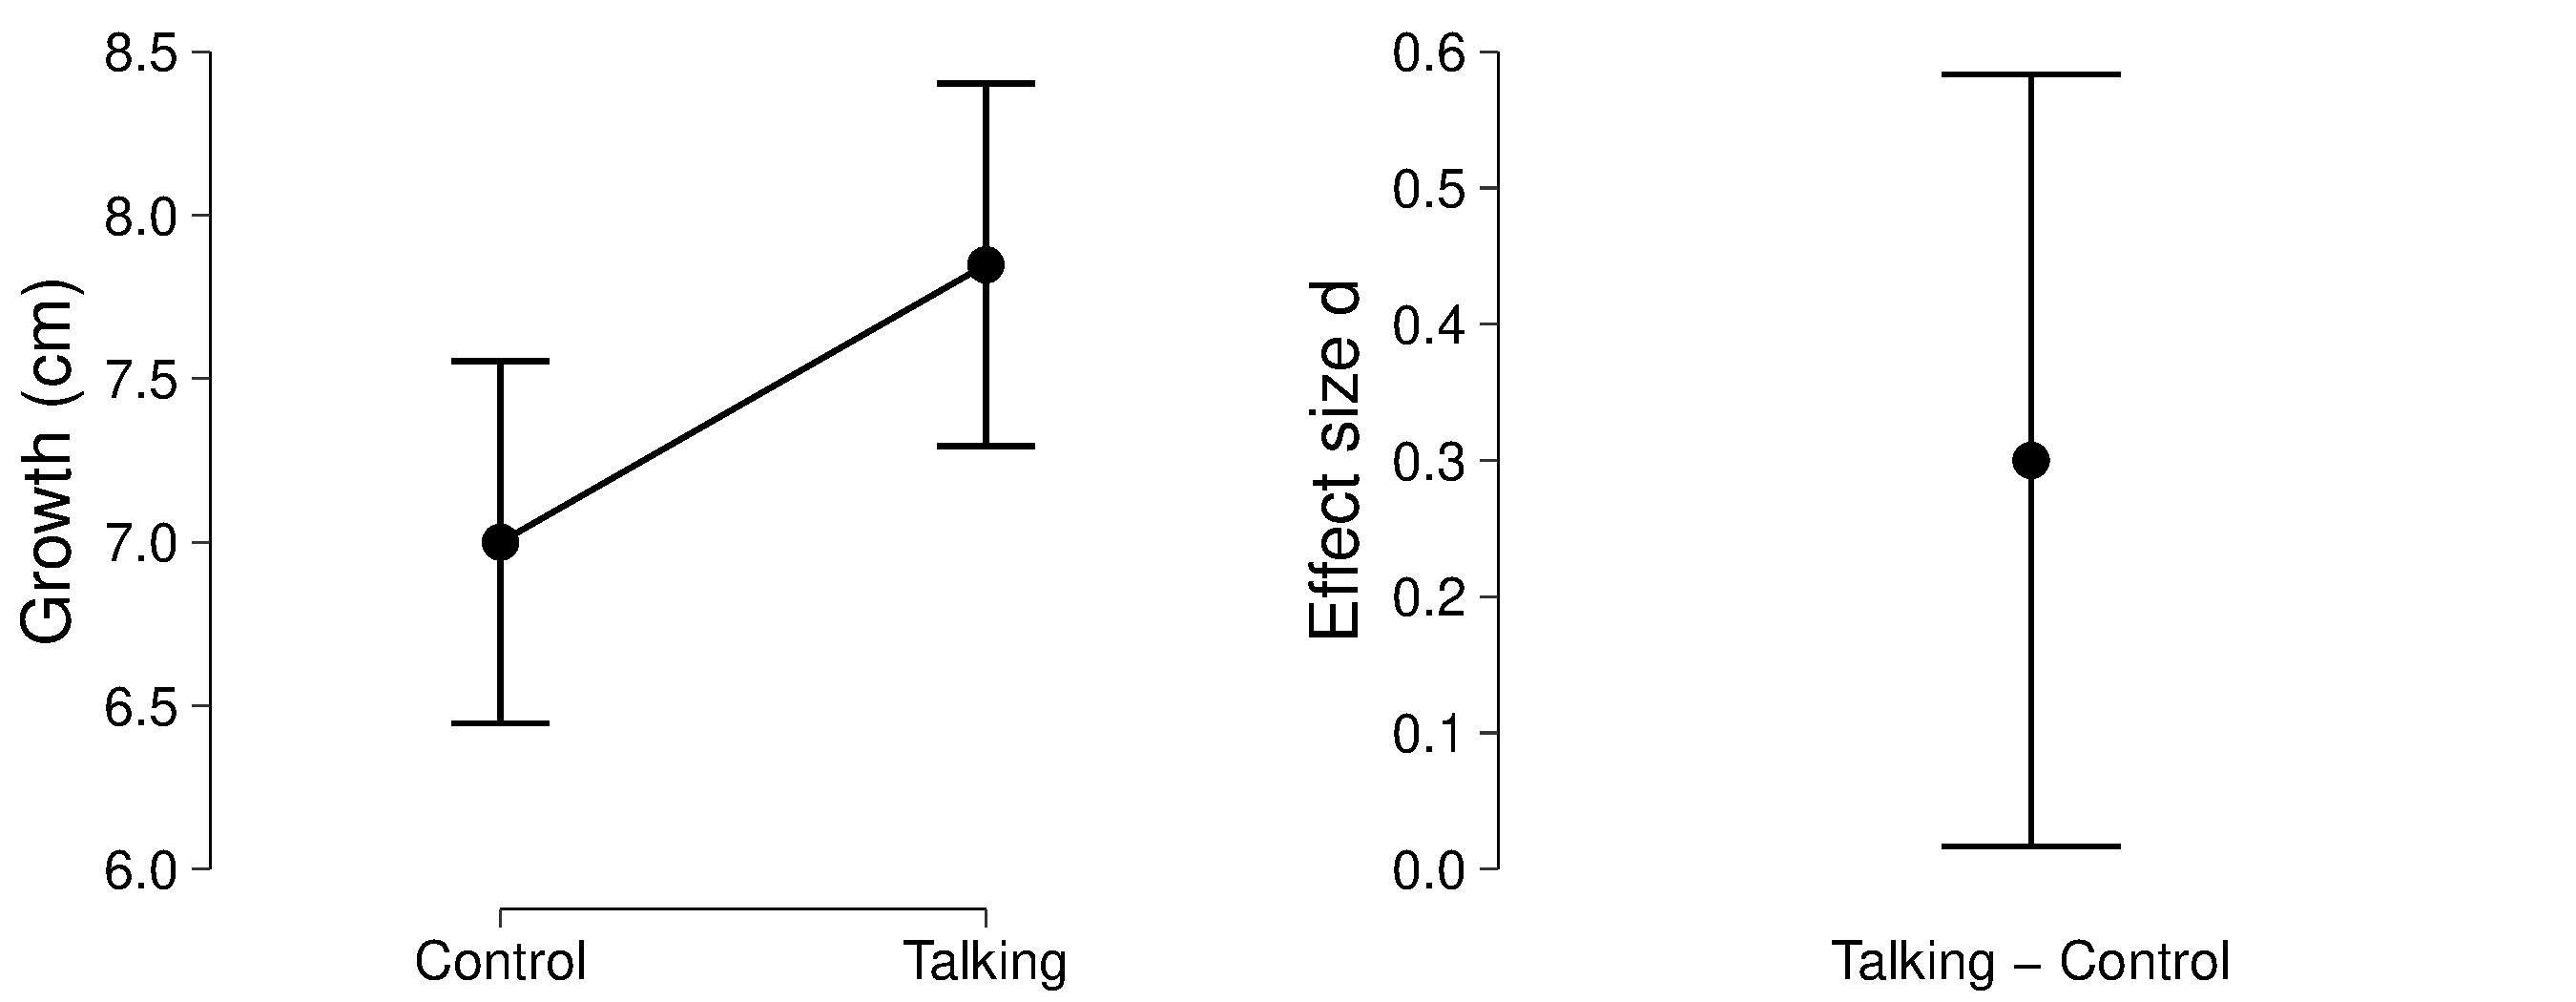
\includegraphics[width=\textwidth]{descriptivesPlot.pdf}
	\caption{Standard estimation results for the fictitious plant growth example. Left panel: a descriptives plot with the mean and 95\% confidence interval of plant growth in the two conditions. Right panel: point estimate and 95\% confidence interval for Cohen's \cohend.}
	\label{fig:descriptivesPlot}
\end{figure}

Based on these results, what would be a reasonable point estimate of effect size? A straightforward and intuitive answer is ``\getValue{0}{Estimate}{\tbEffectSizeExample}''. However, your colleague now informs you of the hypothesis that the experiment was designed to assess: ``plants grow faster when you talk to them''.\footnote{Specifically, imagine your colleague selected 100 plants and weighted them three times: at the start of the experiment, after one week, and after two weeks. The first week 50 plants were randomly selected and spoken to, while the others served as controls. The next week the roles were reversed: the previously spoken to plants served as controls while the control plants were now spoken to. The quantity of interest is the difference in weight between the two conditions. This example is inspired by \protect\citeA{BergerDelampady1987}.} Suddenly, a population effect size of ``0'' appears eminently plausible. Any observed difference may merely be due to the inevitable sampling variability.\footnote{Unless your colleague talked out loud, with consumption, and the plants were near.}

\section*{When Are Effect Sizes Overestimated?}
Standard point estimates and confidence intervals ignore the possibility that the effect is spurious (i.e., the null hypothesis $\mathcal{H}_0$). This is not problematic when $\mathcal{H}_0$ is deeply implausible, either because $\mathcal{H}_0$ was highly unlikely \emph{a priori} or because the data decisively undercut $\mathcal{H}_0$. But when the data fail to undercut $\mathcal{H}_0$, or when $\mathcal{H}_0$ is highly likely \emph{a priori} (i.e., ``plants do not grow faster when you talk to them''), then $\mathcal{H}_0$ is not ruled out as a plausible account of the data. Effect size estimates that ignore a plausible $\mathcal{H}_0$ are generally overconfident: the fact that $\mathcal{H}_0$ provides an acceptable account of the data should shrink effect size estimates towards zero.

\section*{A Spike-and-Slab Perspective}
Here we illustrate both the overestimation and a remedy by reanalyzing the fictitious data from Figure~\ref{fig:descriptivesPlot}.\footnote{R code for the analysis is available at \osflink{}.} We apply the spike-and-slab model \cite{RouderEtAl2018PBR, clyde1996prediction, mitchell1988bayesian}, which consists of two components. The first component corresponds to the position that talking to plants does not affect their growth (i.e., $\delta = 0$), whereas the second component corresponds to the position that speaking to plants does affect their growth (i.e., $\delta \neq 0$). Both components are deemed \emph{a priori} equally likely, such that the prior probability for each component is \nicefrac{1}{2}. Here we view the spike-and-slab setup as a single model, although it can also be viewed as a form of Bayesian model averaging (see Box~\ref{box:box1} for details). In almost all current empirical work, an estimate of effect size is based solely on the second component, which yields a point estimate and an uncertainty interval (for frequentists, $\delta = \getValue{0}{Estimate}{\tbEffectSizeExample}$, 95\%  CI: \getCI{0}{\tbEffectSizeExample}; for Bayesians $\delta = \getValue{1}{mean}{\reanalysis}$, 95\% CRI: \getCI{1}{\reanalysis}). The spike-and-slab model, however, also considers the possibility that an effect can be absent; consequently, the overall estimate from the spike-and-slab model is a weighted average of the two components, shrinking the estimate towards zero.\footnote{For the spike-and-slab model, the posterior distribution is constructed in the following manner: $p(\delta\midd\data) = 1\{\delta = 0\}\prob(\model_0\midd\data) + p(\delta\midd\data,\model_1)\prob(\model_1\midd\data)$. Here, $1\{\delta = 0\}$ is the Dirac delta function which represents the spike under $\mathcal{H}_0$, $\prob$ denotes probability of a model, and $p$ denotes density related to the magnitude of the effect.} Figure 2 contrasts the traditional slab-only estimation against the spike-and-slab estimation.
% these cannot be generated inside the caption
\setValue{0}{ph1}{\reanalysis}{\phAlt}%
\setValue{0}{mode}{\reanalysis}{\modeAlt}%
\begin{figure}[!ht]
	\centering
	\begin{tikzpicture}
		\node[anchor=south west,inner sep=0] (image) at (0,0) {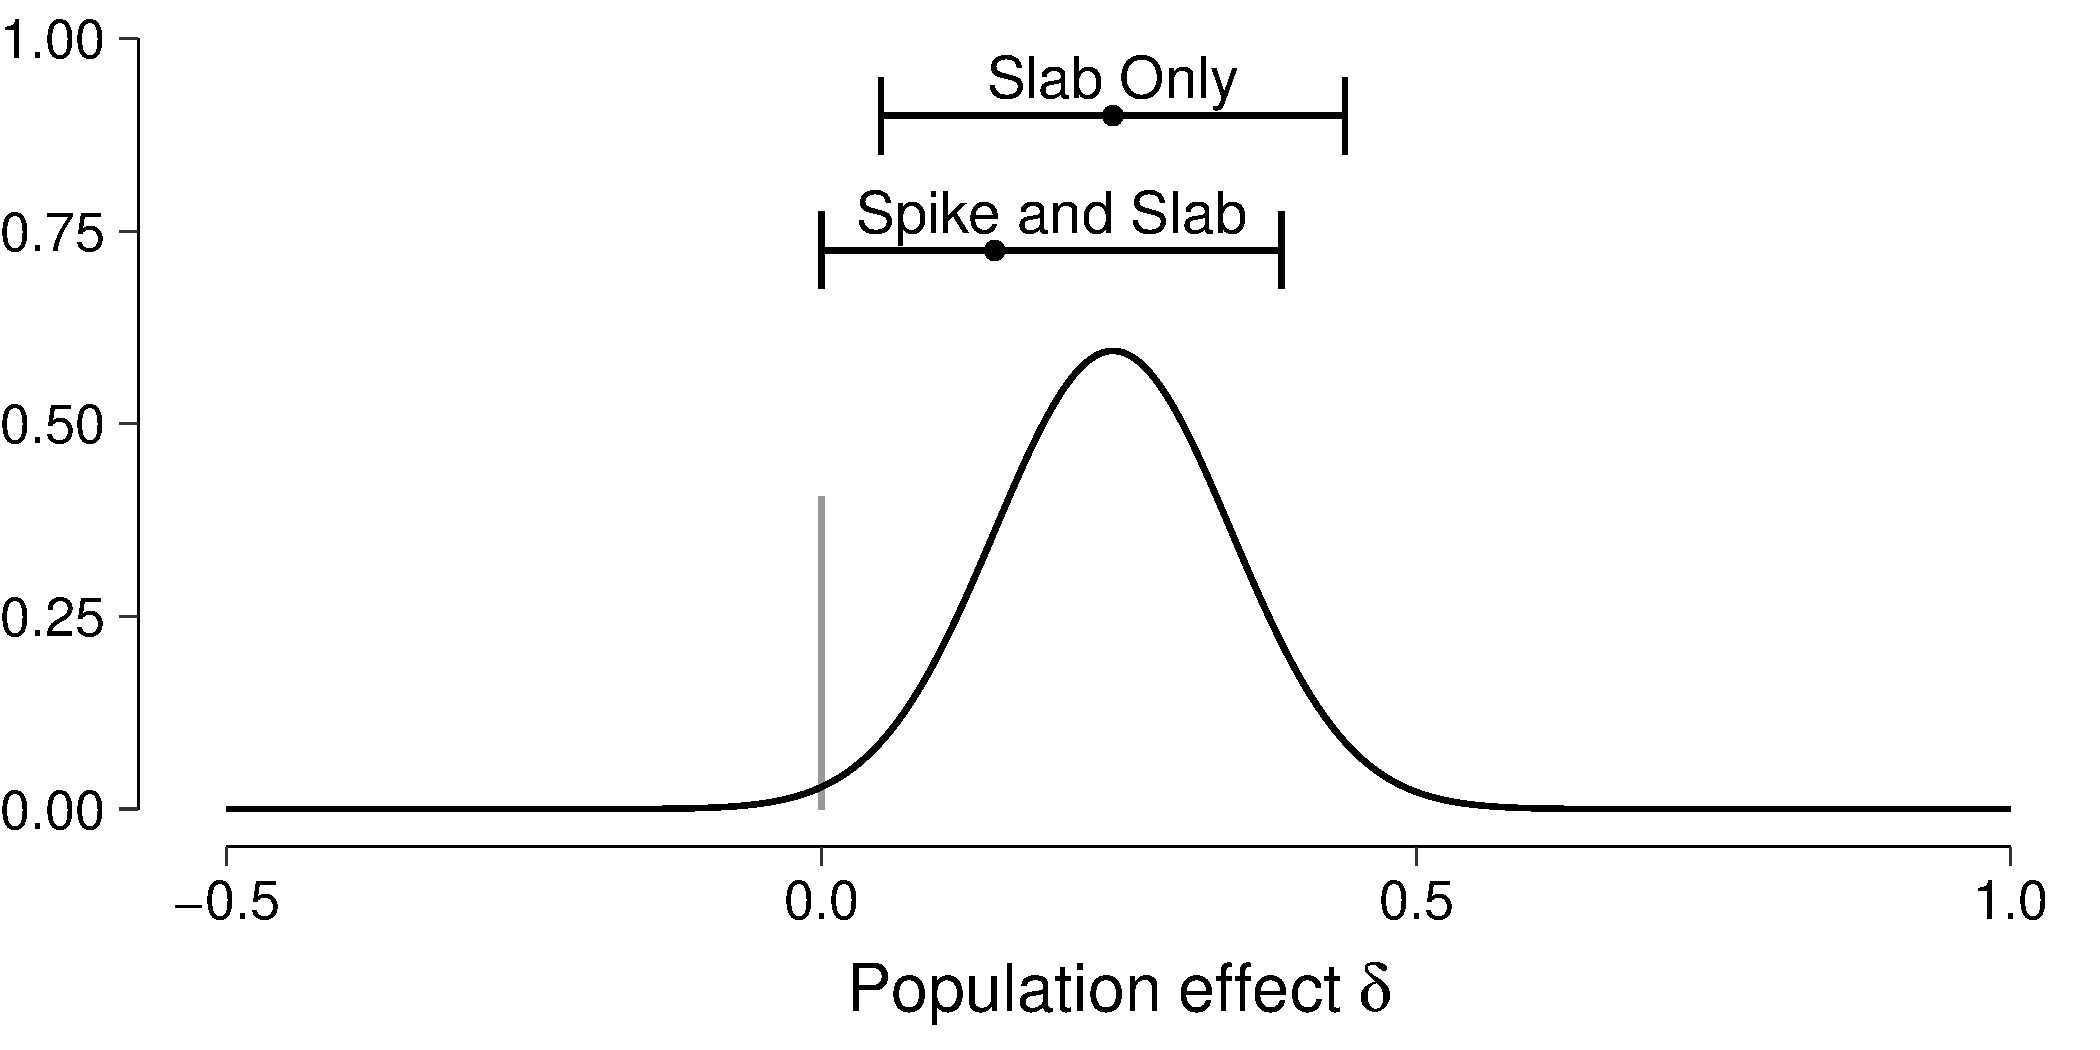
\includegraphics[width=0.9\textwidth]{spikeAndSlabPosteriorRescaledPosteriorMode.pdf}};
		\begin{scope}[x={(image.south east)},y={(image.north west)}]
		\node[anchor=base,inner sep=0pt, outer sep=0pt] at (0.28,0.61) {$p(\hypo{0}\mid\data) = \getValue{0}{ph0}{\reanalysis}$};
		\end{scope}
	\end{tikzpicture}
	\caption{
		The spike-and-slab model. The black line represents the posterior distribution of effect size given the slab (i.e., the effect is non-zero). The posterior is scaled so that its mode ($\delta = \modeAlt$) equals the posterior probability of the alternative model (i.e., $p(\hypo{1}\mid\data) = \phAlt$). The grey line represents the posterior probability of the spike (i.e., $\mathcal{H}_0$: the effect is absent). The error bars and dots above the density show 95\% credible intervals and the posterior mean for the slab-only model and for the spike-and-slab model.}
	\label{fig:modelAveragedPosterior}
\end{figure}
Compared to the traditional results based only on the slab, the posterior mean and central 95\% credible interval of the spike-and-slab model are shrunken towards 0 (i.e., \getValue{0}{mean}{\reanalysis} (95\% CRI: \getCI{0}{\reanalysis}) vs. \getValue{1}{mean}{\reanalysis} (95\% CRI: \getCI{1}{\reanalysis})). This shrinkage is due to the non-negligible probability that the effect is absent. The spike-and-slab posterior represents the plausibility that the effect is absent by the height of the spike, and the uncertainty about the effect's magnitude, given that it is present, by the width of the slab. Note that as the posterior probability of $\mathcal{H}_0$ decreases, the spike-and-slab results approach those of the slab-only model.

\section*{Discussion}
Standard estimates of effect size ignore the null hypothesis and are therefore overconfident, that is, biased away from zero. The spike-and-slab model remedies this problem by explicitly considering the possibility that an effect is absent \cite{Robinson2019,RouderEtAl2018PBR}. The core idea dates back to \citeA{Jeffreys1939}; nonetheless, it is ignored both in empirical practice, in statistical education, and in journal guidelines.

%\subsubsection*{Extending the Null to a Perinull}
\subsubsection*{What if All Null Hypotheses Are False?}
The spike-and-slab approach clashes with the popular estimation mindset, where it is argued that statistical significance should be abandoned in favor of estimation \cite{McShane2019abandon, Cumming2016introduction, valentine2015life, Cumming2014}. One argument to forgo hypothesis testing is that all null hypotheses are false \cite{Cohen1990, Meehl1978} and therefore there is no need to consider a component that states that an effect is exactly zero. The statistical counterargument is that point null hypotheses are merely mathematically convenient approximations to more complex perinull hypotheses that allow mass on an interval close to zero \cite{BergerDelampady1987, KiersTendeiro2019}. Thus, from a pragmatic perspective it is irrelevant whether or not null hypotheses are exactly true: in the spike-and-slab model, a perinull ``stake'' or ``chimney'' \cite{KiersTendeiro2019} component will shrink estimates towards zero almost as much as the point null spike component will. 

\subsubsection*{When to Ignore the Spike}
There are two scenarios in which the presence of the spike (or perinull stake) can safely be ignored. First, the spike may be deeply implausible. This happens most often in problems of pure estimation, such as when determining the relative popularity of two politicians or the proportion of Japanese cars on the streets of New York. In such cases, no value or interval needs to be singled out for special attention. Second, the data may provide overwhelming evidence that an effect is present. When this happens, the results from a spike-and-slab model become virtually identical to those of a slab-only model, and the inclusion of the spike does not offer an added benefit. A practical recommendation by Harold Jeffreys is to ignore the spike whenever sample sizes fall between 50 and 2000 and the maximum likelihood estimate deviates from the spike by more than three standard errors (\citeNP[pp. 193--194]{Jeffreys1939}; \citeNP[p. 75]{Jeffreys1980}).

\subsubsection*{Conclusion}
Standard methods for estimating effect size produce results that are overly optimistic. This bias toward high estimates can be corrected by applying the spike-and-slab model which explicitly accounts for the possibility that the effect is absent. 

\newpage
\begin{NewBox2}[label=box:box1]{The Spike-and-Slab Distribution as Bayesian Model Averaging}{}%
	\vspace{6pt}\hrule\vspace{6pt}
	The spike-and-slab distribution can be viewed as a single model that consists of two components: the slab, which assumes that the effect is present, and the spike, which assumes the effect is absent. However, the spike-and-slab distribution can also be seen as a form of Bayesian model averaging. From that perspective, the spike and the slab are two individual models. The slab represents the unconstrained model that freely estimates effect size, and the spike represents the constrained model where the effect size is fixed to zero. Next, the results for each model are weighted by the posterior model probabilities and averaged, so that inference can be made using results from both models simultaneously. Such averaging over models yields optimal predictive performance (\citeNP[p. 640--641]{ZellnerVandaele1975}, as described in \citeNP[p. 600--601]{ZellnerSiow1980}; \citeNP[p. 57]{Haldane1932}; \citeNP{IversonEtAl2010}; \citeNP{RouderEtAl2018PBR}), and conceptually similar ideas date back much further (\citeNP[p. 387]{WrinchJeffreys1921}; \citeNP{Jevons18741913}). Note that these two perspectives ---a two-component model or averaging of two models--- differ in semantics but are mathematically equivalent.
\end{NewBox2}

\newpage

\bibliographystyle{apacite}
% \bibliography{referenties, referenties.bib}
\bibliography{referenties.bib}

\end{document}